%% Template for a preprint Letter or Article for submission
%% to the journal Nature.
%% Written by Peter Czoschke, 26 February 2004
%%

\documentclass{nature}

%% make sure you have the nature.cls and naturemag.bst files where
%% LaTeX can find them

\bibliographystyle{naturemag}

\title{Coevolution leaves a stronger imprint on interactions than on community structure.}

%% Notice placement of commas and superscripts and use of &
%% in the author list

\author{Timoth\'ee Poisot$^{1}$ \& Daniel B. Stouffer$^1$}


\begin{document}

\maketitle

\begin{affiliations}
 \item School of Biological Sciences, University of Canterbury, Private Bag 4800, Christchurch 8140, New Zealand
\end{affiliations}

\textbf{Coevolutionary dynamics act on both species and their interactions
in ways that shape ecological communities \textsuperscript{1--4}. It
remains unclear, however, how the structure of communities at larger
spatial scales either influences or is influenced by local coevolutionary
processes \textsuperscript{5,6}, and how mechanisms acting at these different
scales feedback onto one another \textsuperscript{7--9}. Here we show that,
although species interactions vary substantially over a continental gradient,
the coevolutionary significance of individual interactions is maintained
across different scales. Notably, this occurs despite the fact that observed
community variation at the local scale frequently tends to weaken or remove
community-wide coevolutionary signal. When considered in terms of the interplay
between community ecology and coevolutionary theory, our results demonstrate
that individual interactions are capable and likely to show a consistent
signature of past coevolution even when woven into communities that do not.}

Ecological interactions often exert important selective pressures on the
species involved. For example, the phenologies of lodgepole pines and red
crossbills respond spatially to the presence of squirrels \textsuperscript{1}
and palm species undergo changes in seed morphology in response to the
extinction of bird dispersing their seeds \textsuperscript{3}. Given that
interactions are distributed in similar ways across communities, at both
the large or small scale \textsuperscript{10}, it can be argued that much
ecological structure is the end result of evolutionary or coevolutionary
dynamics between species \textsuperscript{11,12}. Unfortunately, while
the coevolutionary dynamic of pairs of interacting species has been well
described at macro \textsuperscript{13} and micro \textsuperscript{14}
evolutionary timescales, most attempts to understand how they cascade up
to the levels of diversity of both species and interactions found within
empirical communities have been inconclusive \textsuperscript{15}.  Moreover,
because coevolutionary dynamics are often presented as a key driving force
behind ecological structure across both time and space \textsuperscript{6},
it is crucial to determine the scale at which they are both relevant and
quantifiable.

Historically, the evidence for coevolution in taxonomically diverse communities
is quantified as the degree of matching between the phylogenies of two
sets of interacting organisms \textsuperscript{16}.  This notion builds on
the century-old idea that extant species interact in a way similar to the
way their ancestors did \textsuperscript{17}, but it is considerably more
restrictive than just phylogenetic conservation of species' interactions
\textsuperscript{11,18} because it additional higher-order constraints. More
explicitly, communities that have assembled by successive divergence events
due to coevolution should display phylogenetic congruence, that is (i)
have similar phylogenetic trees and (ii) have species at matching positions
in the trees that tend to interact \textsuperscript{7}. On the other hand,
many ecological and evolutionary processes that occur locally are expected
to blur community-wide coevolutionary signal \textsuperscript{9}. One
possible explanation is that interactions can display substantial turnover
at ecologically relevant temporal and spatial scales \textsuperscript{19}:
the same two species can interact in different ways under the effect of
local environmental contingencies, spatial mismatch in species phenologies,
variations in population abundances, and chance events \textsuperscript{20}. It
is unclear, however, whether these mechanisms influence how the coevolutionary
signal within individual interactions should vary across spatial scales.

To answer these questions, we study a dataset of interactions between rodents
and their ectoparasites from 51 sites across Western to Eastern Europe
\textsuperscript{21} (Methods Summary). This dataset is uniquely suited for
this task as it represents a paradigmatic system in which species-species
interactions are thought to be driven by macro-evolution and co-speciation
events \textsuperscript{22}, and coevolutionary signal is indeed significant
at the continental level \textsuperscript{23} ($p \leq 10^{-4}$; Methods
Summary). Importantly, it also provides spatial replication and variability
at a scale large enough to capture macro-ecological processes.

As host-macroparasite interactions are hypothesized to be both ecologically
constrained and evolutionary conserved \textsuperscript{24}, the congruence
observed at the continental level sets the baseline for what would be
expected in local communities. Of course, if ecological mechanisms reduce
coevolutionary signal, we should detect coevolution at the continental scale
but not locally. Noting that variation of interactions can decrease congruence,
we analyse the data at two different levels to test these hypotheses: first,
we use \emph{regional} interaction data---which accounts for different
species composition across sites--and second, we use the \emph{local}
interaction data---which also accounts for variation in the interactions
between observed these species (Methods Summary). Out of 51 sites, 35 show no
signal of coevolution, 11 show significant coevolutionary signal when using
the regional interactions, and 12 show significant coevolutionary signal
using the local interactions (see \emph{Supp. Mat.} for network-level
significance values).

These results would appear to support the idea that macro-evolutionary
processes such as co-diversification can have consequences at the
macro-ecological level but may not in fact be detectable at finer spatial
scales. On the other hand, system-level differences say little about the
behaviour of individual interactions, despite the fact most coevolutionary
mechanisms act at the interaction level \textsuperscript{25}. As might be
expected, we observe here that networks with interactions that are important
for coevolution at the continental scale indeed have more coevolutionary signal
at the local and regional scales alike (Fig. 2A). Intriguingly, we also find
that the distribution of individual interactions' contributions to coevolution
is strongly conserved, regardless of the scale at which the interactions are
quantified (Fig. 2B). Because interactions differ in their total contribution
to coevolution, this implies that their distribution across networks is what
actually drives differences in overall coevolutionary signal. Network-level
coevolutionary signal emerges directly from the properties of interactions
and is not a property of the network itself.

Beyond their contribution to coevolution, interactions also ultimately
differ in how frequently they vary when the species involved co-occur
\textsuperscript{26}. Once more, the literature on host-parasite
interactions usually assumes that the reason why some interactions are more
frequent is because they reflect a significant past history of coevolution
\textsuperscript{27}. If this were true, we should observe a significant,
positive correlation between the probability of observing an interaction and
the importance of that interaction for coevolution at the continental scale
(Methods Summary). Surprisingly, we find that neither is true here since
interactions that are important for coevolution are not more conserved
(Fig. 3).

Ultimately, coevolutionary signal varies across scale because of the
simultaneous variation of species' interactions \emph{and} communities'
phylogenetic tree structure. In a system characterised by substantial turnover,
we would expect the contribution of each separate interaction to differ across
scales as well. Instead, we observe here that interactions that contribute
strongly to coevolutionary signal at the continental scale \emph{also} show a
significant tendency to contribute strongly at the local ($p<0.05$ for positive
correlations in 48 out of 51 networks) and regional (in 47 out of 51 networks),
and this observation is independent of network-wide coevolutionary signal
(Fig.  4). Remarkably, this result implies that the remnants of coevolution
are still locally detectable in \emph{individual interactions} even though
coevolution regularly fails to leave its imprint on most local networks.

Overall, the results of our analyses demonstrate that there is a sizeable gap
between our current understanding of coevolution as the basis of multi-species
interactions and its applicability to ecological questions. Local networks
show little to no signal of coevolution and the strength of coevolution
between two species is a surprisingly poor predictor of how frequently they
interact. In contrast to the frequent assumption that phylogenetic structure
is a key driver of community structure \textsuperscript{28}, these data
reveal that this impact is actually minimal at ecologically relevant spatial
scales. Despite all the above, individual interactions are able to maintain
their coevolutionary signal even when the community they are woven into does
not. Thinking more broadly, these discrepancies provide a clear roadmap
for bridging the aforementioned gap between our appreciation of the role
of coevolution and its empirically measurable outcomes. Network structure
is the most parsimonious \emph{mechanism} by which coevolution proceeds,
not the imprint coevolution leaves on ecological communities.

\begin{figure}
\centering
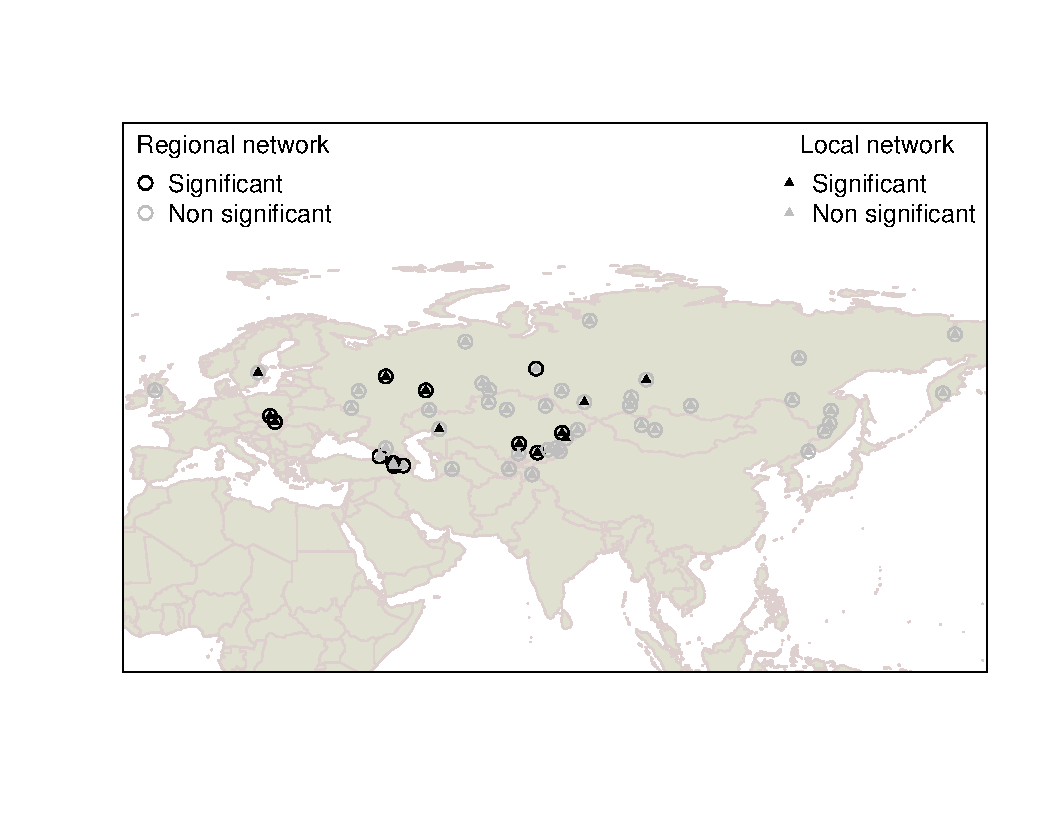
\includegraphics{../figures/figure1.pdf}
\caption{Spatial distribution of coevolutionary signal across the 51
sites. For each location, we indicate whether or not the structure of
regional and local interaction networks is consistent with phylogenetic
congruence. The colour of the circle corresponds to regionally
significant or non-significant (black and grey, respectively) while the
colour of the symbol within corresponds to locally significant or
non-significant (black and grey, respectively).}
\end{figure}

\begin{figure}
\centering
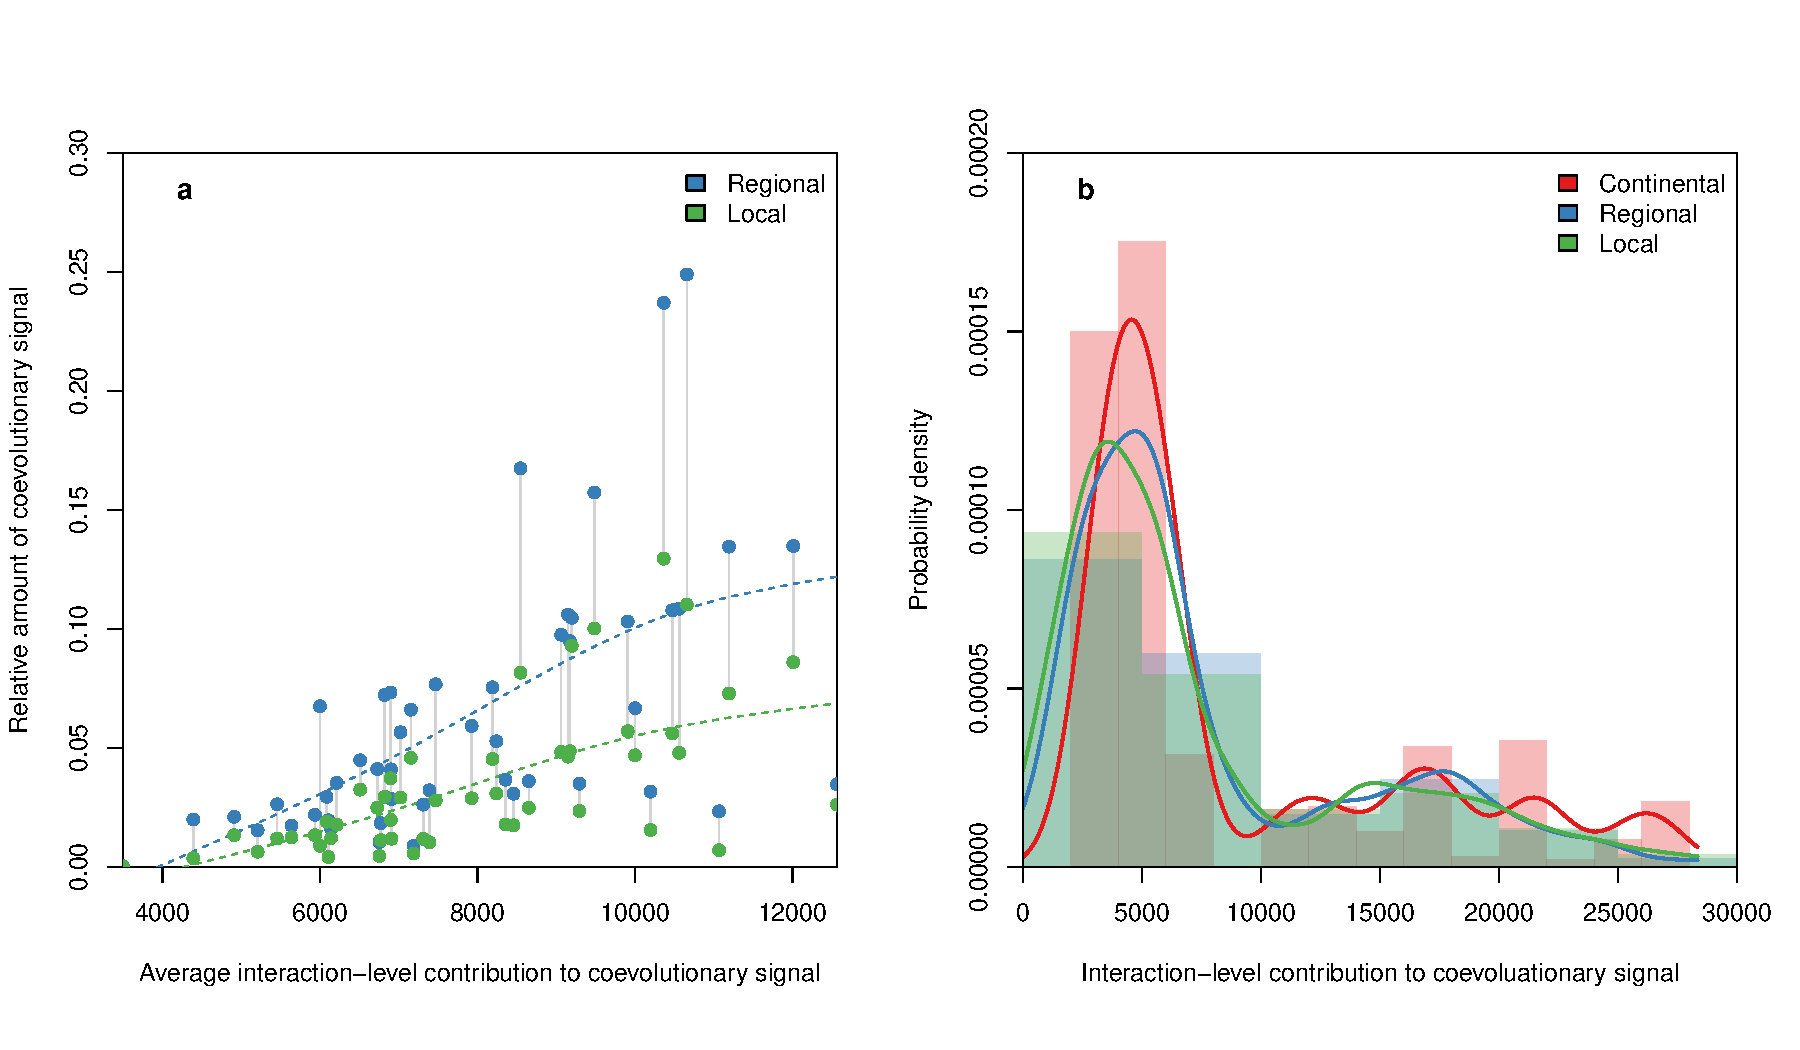
\includegraphics{../figures/figure4.pdf}
\caption{Distribution of coevolutionary signal at the network and
interaction levels. \textbf{a}, Networks that have lower coevolutionary
signal at the local or regional level are composed of interactions that
on average contribute little to coevolution at the continental scale.
Dashed lines are the cubic smoothing spline; the two levels of the same
networks are linked by solid grey lines. \textbf{b}, Overall,
interactions observed at the local, regional, and continental scale have
equal contributions to coevolutionary signal. Probability density was
smoothed using a Gaussian kernel density estimator. Raw probability
densities are shown as semi-transparent bars.}
\end{figure}

\begin{figure}
\centering
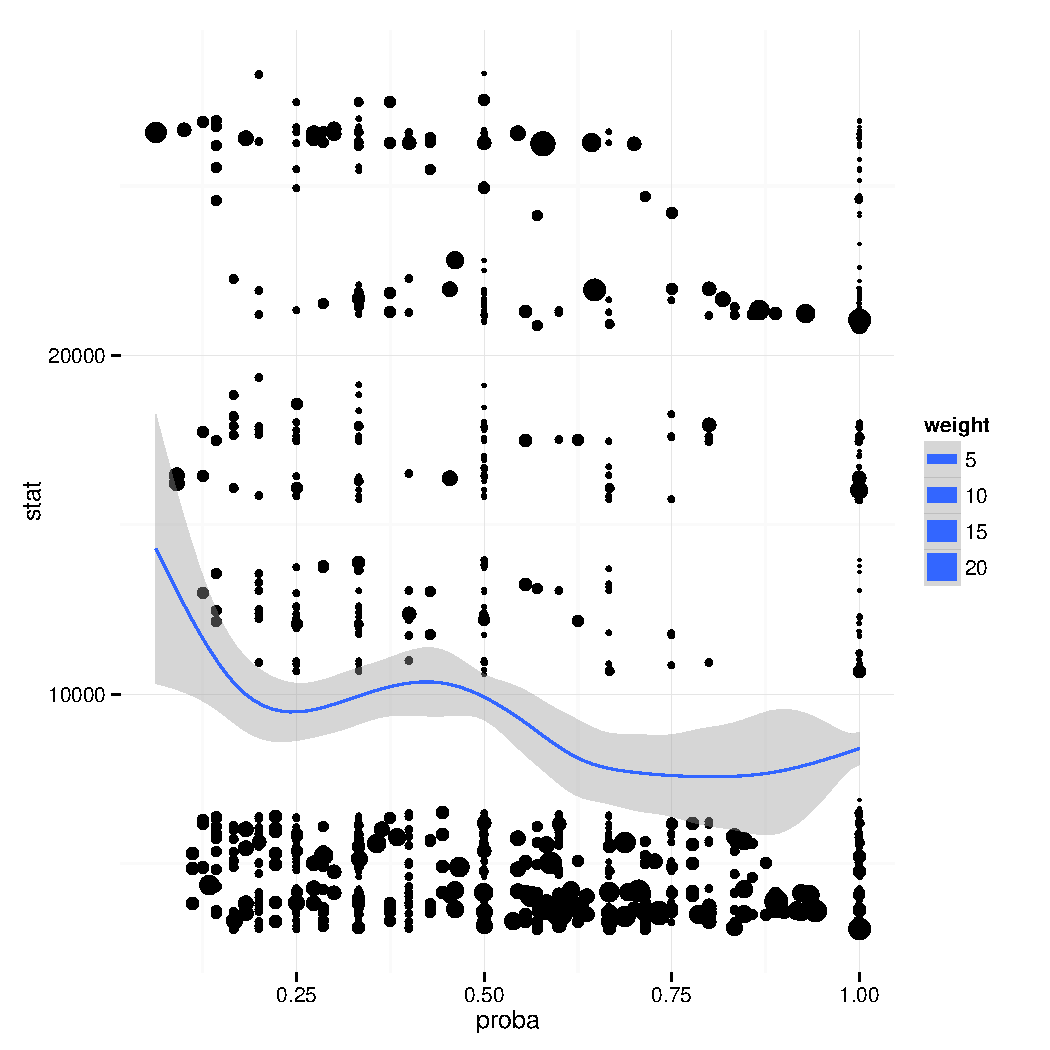
\includegraphics{../figures/figure3.pdf}
\caption{Spatial consistency of an interaction and its contribution to
coevolutionary signal. Spatial consistency is defined as the probability
of observing an interaction between two species given that they were
observed to co-occur. Although statistically significant, there was no
biologically meaningful relationship between spatial consistency and an
interaction's importance for coevolution in the continental network
($R^2 \approx 0.01$, $\rho = -0.1$, $p \leq 10^{-5}$).}
\end{figure}

\begin{figure}
\centering
\includegraphics{../figures/figure2.pdf}
\caption{The contribution to coevolutionary signal of the interaction
between two species is maintained across scales. For every site, we show
the Pearson's correlation between interaction-level coevolutionary
signal in the continental network and the same in the local network. The
size of each point is proportional to the size of the network, and all
correlations are significant at $\alpha = 0.05$ except in the grey
shaded area.}
\end{figure}

\begin{methods}

We use data on observations of interactions between 121 species of
rodents and 205 species of parasitic fleas in 51 locations across Europe
\textsuperscript{21} to build 51 species-species interaction networks.
Interactions were measured by combing rodents for fleas, a method that
gives high quality data as it has a high power of detection. To account
for differential sampling effort and across site variations in
abundance, we only study the networks' incidence matrices (presence and
absence of interactions).

In our study, we define threes scales for the network data and
analysis---continental, regional, and local. The continental scale is
the aggregated ``metanetwork'' which includes all potential interactions
between co-occurring species \textsuperscript{19} (\emph{i.e.}, all
species and all their interactions across the 51 networks). Within each
site, the regional scale is given by the list of observed species and
all their possible interactions. Hence the regional networks are always
a perfect subset of the continental network. The local scale includes
only the interactions that were actually observed in the field at a
given site. Therefore, the local and regional networks always include
the same species, but the local network has only a subset (or, at most,
an exact match) of the interactions in the regional network. The spatial
consistency of every individual interaction is measured as the number of
sites in which the two species involved co-occur.

We quantified the coevolutionary signal in terms of the degree of
matching between host and parasite phylogenies given knowledge of
species interactions using the \emph{PACO} method \textsuperscript{29},
which is robust to variations in number of species. \emph{PACO} provides
measures of both the network-level congruence (\emph{i.e.}, is the
network coevolved?) and the interaction-level signal (\emph{i.e.}, what
is the contribution of each interaction to the overall coevolutionary
signal?). We measured the phylogenetic dissimilarity between two sites
for hosts and parasites using PCD \textsuperscript{30}, a measure that
accounts for the dissimilarity of species, corrected for the
phylogenetic distance between all species in the dataset. Since it is a
requirement of the methods we use here, the phylogenetic trees for hosts
and parasites were rendered ultrametric (i.e., all species are at the
same distance from the root).

\end{methods}

%% Put the bibliography here, most people will use BiBTeX in
%% which case the environment below should be replaced with
%% the \bibliography{} command.

% \begin{thebibliography}{1}
% \bibitem{dummy} Articles are restricted to 50 references, Letters
% to 30.
% \bibitem{dummyb} No compound references -- only one source per
% reference.
% \end{thebibliography}

\section*{References}

\begin{enumerate}

\item Benkman, C. W., Parchman, T. L., Favis, A. \& Siepielski, A.
M. Reciprocal selection causes a coevolutionary arms race
between crossbills and lodgepole pine. \emph{Am. Nat.} \textbf{162,}
182--194 (2003).

\item Thompson, J. N. The coevolving web of life. \emph{Am.
Nat.} \textbf{173,} 125--140 (2009).

\item Galetti, M. \emph{et al.} Functional Extinction of Birds Drives Rapid
Evolutionary Changes in Seed Size. \emph{Science} \textbf{340,}
1086--1090 (2013).

\item Nuismer, S. L., Jordano, P. \& Bascompte, J. Coevolution
and the Architecture of Mutualistic Networks. \emph{Evolution}
\textbf{67,} 338--354 (2013).

\item Nuismer, S. L., Thompson, J. N. \& Gomulkiewicz, R.
Coevolution between hosts and parasites with partially overlapping
geographic ranges. \emph{J. Evol. Biol.} \textbf{16,} 1337--1345 (2003).

\item Thompson, J. N. \emph{The Geographic Mosaic of
Coevolution}. (University Of Chicago Press, 2005).

\item Page, R. D. M. \emph{Tangled trees: Phylogeny,
cospeciation, and coevolution}. (University of Chicago Press, 2003).

\item Urban, M. C. \emph{et al.} The evolutionary ecology of
metacommunities. \emph{Trends Ecol. Evol.} \textbf{23,} 311--317 (2008).

\item Poisot, T. in \emph{Evolutionary Ecology of
Host-Parasite Systems} (eds. Morand, S., Littlewood, D. T. \& Poulin,
R.) (Cambridge University Press, 2015).

\item Jordano, P., Bascompte, J. \& Olesen, J. M. Invariant
properties in coevolutionary networks of plant-animal interactions.
\emph{Ecol. Lett.} \textbf{6,} 69--81 (2003).

\item Eklof, A., Helmus, M. R., Moore, M. \& Allesina, S. Relevance of
evolutionary history for food web structure. \emph{Proc. R. Soc. B Biol. Sci.}
\textbf{279,} 1588--1596 (2011).

\item Stouffer, D. B., Sales-Pardo, M., Sirer, M. I. \& Bascompte,
J. Evolutionary Conservation of Species' Roles in Food
Webs. \emph{Science} \textbf{335,} 1489--1492 (2012).

\item Van Valen, L. A new evolutionary law. \emph{Evol.
Theory} \textbf{1,} 1--30 (1973).

\item Gandon, S., Buckling, A., Decaestecker, E. \& Day, T.
Host-parasite coevolution and patterns of adaptation across time and
space. \emph{J. Evol. Biol.} \textbf{21,} 1861--1866 (2008).

\item Hembry, D. H., Yoder, J. B. \& Goodman, K. R.
Coevolution and the Diversification of Life. \emph{The American
Naturalist} \textbf{184,} 425--438 (2014).

\item Legendre, P., Desdevises, Y. \& Bazin, E. A statistical
test for host-parasite coevolution. \emph{Syst. Biol.} \textbf{51,}
217--234 (2002).

\item Fahrenholz, H. Ectoparasiten und abstammungslehre.
\emph{Zool. Anz.} \textbf{41,} 371--374 (1913).

\item Rezende, E. L., Lavabre, J. E., Guimarães, P. R., Jordano, P. \&
Bascompte, J. Non-random coextinctions in phylogenetically
structured mutualistic networks. \emph{Nature} \textbf{448,} 925--8
(2007).

\item Poisot, T., Canard, E., Mouillot, D., Mouquet, N. \& Gravel,
D. The dissimilarity of species interaction networks.
\emph{Ecol Lett} \textbf{15,} 1353--1361 (2012).

\item Poisot, T., Stouffer, D. B. \& Gravel, D. Beyond
species: why ecological interaction networks vary through space and
time. \emph{Oikos} n/a--n/a (2014).

\item Krasnov, B. \emph{et al.} Data from: Phylogenetic signal in module
composition and species connectivity in compartmentalized host-parasite
networks. \emph{Data Dryad} \texttt{10255/dryad.36193} (2012).

\item Verneau, O., Du Preez, L. \& Badets, M. Lessons from
parasitic flatworms about evolution and historical biogeography of their
vertebrate hosts. \emph{C. R. Biol.} \textbf{332,} 149--158 (2009).

\item Krasnov, B. R. \emph{et al.} Phylogenetic Signal in Module
Composition and Species Connectivity in Compartmentalized Host-Parasite
Networks. \emph{Am. Nat.} \textbf{179,} 501--511 (2012).

\item Combes, C. \emph{Parasitism - The Ecology and Evolution
of Intimate Interactions}. (University Of Chicago Press, 2001).

\item Thompson, J. N. The raw material for coevolution.
\emph{Oikos} \textbf{84,} 5--16 (1999).

\item Olito, C. \& Fox, J. W. Species traits and abundances
predict metrics of plant--pollinator network structure, but not pairwise
interactions. \emph{Oikos} n/a--n/a (2014).

\item Morand, S. \& Krasnov, B. \emph{Biogreography of host-parasite
interactions}. (Oxford University Press, 2010).

\item Cavender-Bares, J., Kozak, K. H., Fine, P. V. A. \& Kembel, S.
W. The merging of community ecology and phylogenetic
biology. \emph{Ecol. Lett.} \textbf{12,} 693--715 (2009).

\item Balbuena, J. A., Míguez-Lozano, R. \& Blasco-Costa, I. \emph{et al.}
PACo: A Novel Procrustes Application to Cophylogenetic Analysis.
\emph{PLoS ONE} \textbf{8,} e61048 (2013).

\item Ives, A. R. \& Helmus, M. R. Phylogenetic Metrics of
Community Similarity. \emph{The American Naturalist} \textbf{176,}
E128--E142 (2010).

\end{enumerate}

%% Here is the endmatter stuff: Supplementary Info, etc.
%% Use \item's to separate, default label is "Acknowledgements"

\begin{addendum}
 \item We thank Juan Antonio Balbuena for
discussions about the \emph{PACo} method, and members of the Stouffer
and Tylianakis groups for comments on an early draft of this manuscript.
Funding to TP and DBS was provided by a Marsden Fund Fast-Start grant
(UOC-1101) and to DBS by a Rutherford Discovery Fellowship, both
administered by the Royal Society of New Zealand.
 \item[Competing Interests] The authors declare that they have no
competing financial interests.
 \item[Correspondence] Correspondence and requests for materials
should be addressed to T.P.~(email: tim@poisotlab.io).
\end{addendum}

\end{document}
